
\documentclass{article} % For LaTeX2e
\usepackage{iclr2020_conference,times}

% Optional math commands from https://github.com/goodfeli/dlbook_notation.
%%%%% NEW MATH DEFINITIONS %%%%%

\usepackage{amsmath,amsfonts,bm}

% Mark sections of captions for referring to divisions of figures
\newcommand{\figleft}{{\em (Left)}}
\newcommand{\figcenter}{{\em (Center)}}
\newcommand{\figright}{{\em (Right)}}
\newcommand{\figtop}{{\em (Top)}}
\newcommand{\figbottom}{{\em (Bottom)}}
\newcommand{\captiona}{{\em (a)}}
\newcommand{\captionb}{{\em (b)}}
\newcommand{\captionc}{{\em (c)}}
\newcommand{\captiond}{{\em (d)}}

% Highlight a newly defined term
\newcommand{\newterm}[1]{{\bf #1}}


% Figure reference, lower-case.
\def\figref#1{figure~\ref{#1}}
% Figure reference, capital. For start of sentence
\def\Figref#1{Figure~\ref{#1}}
\def\twofigref#1#2{figures \ref{#1} and \ref{#2}}
\def\quadfigref#1#2#3#4{figures \ref{#1}, \ref{#2}, \ref{#3} and \ref{#4}}
% Section reference, lower-case.
\def\secref#1{section~\ref{#1}}
% Section reference, capital.
\def\Secref#1{Section~\ref{#1}}
% Reference to two sections.
\def\twosecrefs#1#2{sections \ref{#1} and \ref{#2}}
% Reference to three sections.
\def\secrefs#1#2#3{sections \ref{#1}, \ref{#2} and \ref{#3}}
% Reference to an equation, lower-case.
\def\eqref#1{equation~\ref{#1}}
% Reference to an equation, upper case
\def\Eqref#1{Equation~\ref{#1}}
% A raw reference to an equation---avoid using if possible
\def\plaineqref#1{\ref{#1}}
% Reference to a chapter, lower-case.
\def\chapref#1{chapter~\ref{#1}}
% Reference to an equation, upper case.
\def\Chapref#1{Chapter~\ref{#1}}
% Reference to a range of chapters
\def\rangechapref#1#2{chapters\ref{#1}--\ref{#2}}
% Reference to an algorithm, lower-case.
\def\algref#1{algorithm~\ref{#1}}
% Reference to an algorithm, upper case.
\def\Algref#1{Algorithm~\ref{#1}}
\def\twoalgref#1#2{algorithms \ref{#1} and \ref{#2}}
\def\Twoalgref#1#2{Algorithms \ref{#1} and \ref{#2}}
% Reference to a part, lower case
\def\partref#1{part~\ref{#1}}
% Reference to a part, upper case
\def\Partref#1{Part~\ref{#1}}
\def\twopartref#1#2{parts \ref{#1} and \ref{#2}}

\def\ceil#1{\lceil #1 \rceil}
\def\floor#1{\lfloor #1 \rfloor}
\def\1{\bm{1}}
\newcommand{\train}{\mathcal{D}}
\newcommand{\valid}{\mathcal{D_{\mathrm{valid}}}}
\newcommand{\test}{\mathcal{D_{\mathrm{test}}}}

\def\eps{{\epsilon}}


% Random variables
\def\reta{{\textnormal{$\eta$}}}
\def\ra{{\textnormal{a}}}
\def\rb{{\textnormal{b}}}
\def\rc{{\textnormal{c}}}
\def\rd{{\textnormal{d}}}
\def\re{{\textnormal{e}}}
\def\rf{{\textnormal{f}}}
\def\rg{{\textnormal{g}}}
\def\rh{{\textnormal{h}}}
\def\ri{{\textnormal{i}}}
\def\rj{{\textnormal{j}}}
\def\rk{{\textnormal{k}}}
\def\rl{{\textnormal{l}}}
% rm is already a command, just don't name any random variables m
\def\rn{{\textnormal{n}}}
\def\ro{{\textnormal{o}}}
\def\rp{{\textnormal{p}}}
\def\rq{{\textnormal{q}}}
\def\rr{{\textnormal{r}}}
\def\rs{{\textnormal{s}}}
\def\rt{{\textnormal{t}}}
\def\ru{{\textnormal{u}}}
\def\rv{{\textnormal{v}}}
\def\rw{{\textnormal{w}}}
\def\rx{{\textnormal{x}}}
\def\ry{{\textnormal{y}}}
\def\rz{{\textnormal{z}}}

% Random vectors
\def\rvepsilon{{\mathbf{\epsilon}}}
\def\rvtheta{{\mathbf{\theta}}}
\def\rva{{\mathbf{a}}}
\def\rvb{{\mathbf{b}}}
\def\rvc{{\mathbf{c}}}
\def\rvd{{\mathbf{d}}}
\def\rve{{\mathbf{e}}}
\def\rvf{{\mathbf{f}}}
\def\rvg{{\mathbf{g}}}
\def\rvh{{\mathbf{h}}}
\def\rvu{{\mathbf{i}}}
\def\rvj{{\mathbf{j}}}
\def\rvk{{\mathbf{k}}}
\def\rvl{{\mathbf{l}}}
\def\rvm{{\mathbf{m}}}
\def\rvn{{\mathbf{n}}}
\def\rvo{{\mathbf{o}}}
\def\rvp{{\mathbf{p}}}
\def\rvq{{\mathbf{q}}}
\def\rvr{{\mathbf{r}}}
\def\rvs{{\mathbf{s}}}
\def\rvt{{\mathbf{t}}}
\def\rvu{{\mathbf{u}}}
\def\rvv{{\mathbf{v}}}
\def\rvw{{\mathbf{w}}}
\def\rvx{{\mathbf{x}}}
\def\rvy{{\mathbf{y}}}
\def\rvz{{\mathbf{z}}}

% Elements of random vectors
\def\erva{{\textnormal{a}}}
\def\ervb{{\textnormal{b}}}
\def\ervc{{\textnormal{c}}}
\def\ervd{{\textnormal{d}}}
\def\erve{{\textnormal{e}}}
\def\ervf{{\textnormal{f}}}
\def\ervg{{\textnormal{g}}}
\def\ervh{{\textnormal{h}}}
\def\ervi{{\textnormal{i}}}
\def\ervj{{\textnormal{j}}}
\def\ervk{{\textnormal{k}}}
\def\ervl{{\textnormal{l}}}
\def\ervm{{\textnormal{m}}}
\def\ervn{{\textnormal{n}}}
\def\ervo{{\textnormal{o}}}
\def\ervp{{\textnormal{p}}}
\def\ervq{{\textnormal{q}}}
\def\ervr{{\textnormal{r}}}
\def\ervs{{\textnormal{s}}}
\def\ervt{{\textnormal{t}}}
\def\ervu{{\textnormal{u}}}
\def\ervv{{\textnormal{v}}}
\def\ervw{{\textnormal{w}}}
\def\ervx{{\textnormal{x}}}
\def\ervy{{\textnormal{y}}}
\def\ervz{{\textnormal{z}}}

% Random matrices
\def\rmA{{\mathbf{A}}}
\def\rmB{{\mathbf{B}}}
\def\rmC{{\mathbf{C}}}
\def\rmD{{\mathbf{D}}}
\def\rmE{{\mathbf{E}}}
\def\rmF{{\mathbf{F}}}
\def\rmG{{\mathbf{G}}}
\def\rmH{{\mathbf{H}}}
\def\rmI{{\mathbf{I}}}
\def\rmJ{{\mathbf{J}}}
\def\rmK{{\mathbf{K}}}
\def\rmL{{\mathbf{L}}}
\def\rmM{{\mathbf{M}}}
\def\rmN{{\mathbf{N}}}
\def\rmO{{\mathbf{O}}}
\def\rmP{{\mathbf{P}}}
\def\rmQ{{\mathbf{Q}}}
\def\rmR{{\mathbf{R}}}
\def\rmS{{\mathbf{S}}}
\def\rmT{{\mathbf{T}}}
\def\rmU{{\mathbf{U}}}
\def\rmV{{\mathbf{V}}}
\def\rmW{{\mathbf{W}}}
\def\rmX{{\mathbf{X}}}
\def\rmY{{\mathbf{Y}}}
\def\rmZ{{\mathbf{Z}}}

% Elements of random matrices
\def\ermA{{\textnormal{A}}}
\def\ermB{{\textnormal{B}}}
\def\ermC{{\textnormal{C}}}
\def\ermD{{\textnormal{D}}}
\def\ermE{{\textnormal{E}}}
\def\ermF{{\textnormal{F}}}
\def\ermG{{\textnormal{G}}}
\def\ermH{{\textnormal{H}}}
\def\ermI{{\textnormal{I}}}
\def\ermJ{{\textnormal{J}}}
\def\ermK{{\textnormal{K}}}
\def\ermL{{\textnormal{L}}}
\def\ermM{{\textnormal{M}}}
\def\ermN{{\textnormal{N}}}
\def\ermO{{\textnormal{O}}}
\def\ermP{{\textnormal{P}}}
\def\ermQ{{\textnormal{Q}}}
\def\ermR{{\textnormal{R}}}
\def\ermS{{\textnormal{S}}}
\def\ermT{{\textnormal{T}}}
\def\ermU{{\textnormal{U}}}
\def\ermV{{\textnormal{V}}}
\def\ermW{{\textnormal{W}}}
\def\ermX{{\textnormal{X}}}
\def\ermY{{\textnormal{Y}}}
\def\ermZ{{\textnormal{Z}}}

% Vectors
\def\vzero{{\bm{0}}}
\def\vone{{\bm{1}}}
\def\vmu{{\bm{\mu}}}
\def\vtheta{{\bm{\theta}}}
\def\va{{\bm{a}}}
\def\vb{{\bm{b}}}
\def\vc{{\bm{c}}}
\def\vd{{\bm{d}}}
\def\ve{{\bm{e}}}
\def\vf{{\bm{f}}}
\def\vg{{\bm{g}}}
\def\vh{{\bm{h}}}
\def\vi{{\bm{i}}}
\def\vj{{\bm{j}}}
\def\vk{{\bm{k}}}
\def\vl{{\bm{l}}}
\def\vm{{\bm{m}}}
\def\vn{{\bm{n}}}
\def\vo{{\bm{o}}}
\def\vp{{\bm{p}}}
\def\vq{{\bm{q}}}
\def\vr{{\bm{r}}}
\def\vs{{\bm{s}}}
\def\vt{{\bm{t}}}
\def\vu{{\bm{u}}}
\def\vv{{\bm{v}}}
\def\vw{{\bm{w}}}
\def\vx{{\bm{x}}}
\def\vy{{\bm{y}}}
\def\vz{{\bm{z}}}

% Elements of vectors
\def\evalpha{{\alpha}}
\def\evbeta{{\beta}}
\def\evepsilon{{\epsilon}}
\def\evlambda{{\lambda}}
\def\evomega{{\omega}}
\def\evmu{{\mu}}
\def\evpsi{{\psi}}
\def\evsigma{{\sigma}}
\def\evtheta{{\theta}}
\def\eva{{a}}
\def\evb{{b}}
\def\evc{{c}}
\def\evd{{d}}
\def\eve{{e}}
\def\evf{{f}}
\def\evg{{g}}
\def\evh{{h}}
\def\evi{{i}}
\def\evj{{j}}
\def\evk{{k}}
\def\evl{{l}}
\def\evm{{m}}
\def\evn{{n}}
\def\evo{{o}}
\def\evp{{p}}
\def\evq{{q}}
\def\evr{{r}}
\def\evs{{s}}
\def\evt{{t}}
\def\evu{{u}}
\def\evv{{v}}
\def\evw{{w}}
\def\evx{{x}}
\def\evy{{y}}
\def\evz{{z}}

% Matrix
\def\mA{{\bm{A}}}
\def\mB{{\bm{B}}}
\def\mC{{\bm{C}}}
\def\mD{{\bm{D}}}
\def\mE{{\bm{E}}}
\def\mF{{\bm{F}}}
\def\mG{{\bm{G}}}
\def\mH{{\bm{H}}}
\def\mI{{\bm{I}}}
\def\mJ{{\bm{J}}}
\def\mK{{\bm{K}}}
\def\mL{{\bm{L}}}
\def\mM{{\bm{M}}}
\def\mN{{\bm{N}}}
\def\mO{{\bm{O}}}
\def\mP{{\bm{P}}}
\def\mQ{{\bm{Q}}}
\def\mR{{\bm{R}}}
\def\mS{{\bm{S}}}
\def\mT{{\bm{T}}}
\def\mU{{\bm{U}}}
\def\mV{{\bm{V}}}
\def\mW{{\bm{W}}}
\def\mX{{\bm{X}}}
\def\mY{{\bm{Y}}}
\def\mZ{{\bm{Z}}}
\def\mBeta{{\bm{\beta}}}
\def\mPhi{{\bm{\Phi}}}
\def\mLambda{{\bm{\Lambda}}}
\def\mSigma{{\bm{\Sigma}}}

% Tensor
\DeclareMathAlphabet{\mathsfit}{\encodingdefault}{\sfdefault}{m}{sl}
\SetMathAlphabet{\mathsfit}{bold}{\encodingdefault}{\sfdefault}{bx}{n}
\newcommand{\tens}[1]{\bm{\mathsfit{#1}}}
\def\tA{{\tens{A}}}
\def\tB{{\tens{B}}}
\def\tC{{\tens{C}}}
\def\tD{{\tens{D}}}
\def\tE{{\tens{E}}}
\def\tF{{\tens{F}}}
\def\tG{{\tens{G}}}
\def\tH{{\tens{H}}}
\def\tI{{\tens{I}}}
\def\tJ{{\tens{J}}}
\def\tK{{\tens{K}}}
\def\tL{{\tens{L}}}
\def\tM{{\tens{M}}}
\def\tN{{\tens{N}}}
\def\tO{{\tens{O}}}
\def\tP{{\tens{P}}}
\def\tQ{{\tens{Q}}}
\def\tR{{\tens{R}}}
\def\tS{{\tens{S}}}
\def\tT{{\tens{T}}}
\def\tU{{\tens{U}}}
\def\tV{{\tens{V}}}
\def\tW{{\tens{W}}}
\def\tX{{\tens{X}}}
\def\tY{{\tens{Y}}}
\def\tZ{{\tens{Z}}}


% Graph
\def\gA{{\mathcal{A}}}
\def\gB{{\mathcal{B}}}
\def\gC{{\mathcal{C}}}
\def\gD{{\mathcal{D}}}
\def\gE{{\mathcal{E}}}
\def\gF{{\mathcal{F}}}
\def\gG{{\mathcal{G}}}
\def\gH{{\mathcal{H}}}
\def\gI{{\mathcal{I}}}
\def\gJ{{\mathcal{J}}}
\def\gK{{\mathcal{K}}}
\def\gL{{\mathcal{L}}}
\def\gM{{\mathcal{M}}}
\def\gN{{\mathcal{N}}}
\def\gO{{\mathcal{O}}}
\def\gP{{\mathcal{P}}}
\def\gQ{{\mathcal{Q}}}
\def\gR{{\mathcal{R}}}
\def\gS{{\mathcal{S}}}
\def\gT{{\mathcal{T}}}
\def\gU{{\mathcal{U}}}
\def\gV{{\mathcal{V}}}
\def\gW{{\mathcal{W}}}
\def\gX{{\mathcal{X}}}
\def\gY{{\mathcal{Y}}}
\def\gZ{{\mathcal{Z}}}

% Sets
\def\sA{{\mathbb{A}}}
\def\sB{{\mathbb{B}}}
\def\sC{{\mathbb{C}}}
\def\sD{{\mathbb{D}}}
% Don't use a set called E, because this would be the same as our symbol
% for expectation.
\def\sF{{\mathbb{F}}}
\def\sG{{\mathbb{G}}}
\def\sH{{\mathbb{H}}}
\def\sI{{\mathbb{I}}}
\def\sJ{{\mathbb{J}}}
\def\sK{{\mathbb{K}}}
\def\sL{{\mathbb{L}}}
\def\sM{{\mathbb{M}}}
\def\sN{{\mathbb{N}}}
\def\sO{{\mathbb{O}}}
\def\sP{{\mathbb{P}}}
\def\sQ{{\mathbb{Q}}}
\def\sR{{\mathbb{R}}}
\def\sS{{\mathbb{S}}}
\def\sT{{\mathbb{T}}}
\def\sU{{\mathbb{U}}}
\def\sV{{\mathbb{V}}}
\def\sW{{\mathbb{W}}}
\def\sX{{\mathbb{X}}}
\def\sY{{\mathbb{Y}}}
\def\sZ{{\mathbb{Z}}}

% Entries of a matrix
\def\emLambda{{\Lambda}}
\def\emA{{A}}
\def\emB{{B}}
\def\emC{{C}}
\def\emD{{D}}
\def\emE{{E}}
\def\emF{{F}}
\def\emG{{G}}
\def\emH{{H}}
\def\emI{{I}}
\def\emJ{{J}}
\def\emK{{K}}
\def\emL{{L}}
\def\emM{{M}}
\def\emN{{N}}
\def\emO{{O}}
\def\emP{{P}}
\def\emQ{{Q}}
\def\emR{{R}}
\def\emS{{S}}
\def\emT{{T}}
\def\emU{{U}}
\def\emV{{V}}
\def\emW{{W}}
\def\emX{{X}}
\def\emY{{Y}}
\def\emZ{{Z}}
\def\emSigma{{\Sigma}}

% entries of a tensor
% Same font as tensor, without \bm wrapper
\newcommand{\etens}[1]{\mathsfit{#1}}
\def\etLambda{{\etens{\Lambda}}}
\def\etA{{\etens{A}}}
\def\etB{{\etens{B}}}
\def\etC{{\etens{C}}}
\def\etD{{\etens{D}}}
\def\etE{{\etens{E}}}
\def\etF{{\etens{F}}}
\def\etG{{\etens{G}}}
\def\etH{{\etens{H}}}
\def\etI{{\etens{I}}}
\def\etJ{{\etens{J}}}
\def\etK{{\etens{K}}}
\def\etL{{\etens{L}}}
\def\etM{{\etens{M}}}
\def\etN{{\etens{N}}}
\def\etO{{\etens{O}}}
\def\etP{{\etens{P}}}
\def\etQ{{\etens{Q}}}
\def\etR{{\etens{R}}}
\def\etS{{\etens{S}}}
\def\etT{{\etens{T}}}
\def\etU{{\etens{U}}}
\def\etV{{\etens{V}}}
\def\etW{{\etens{W}}}
\def\etX{{\etens{X}}}
\def\etY{{\etens{Y}}}
\def\etZ{{\etens{Z}}}

% The true underlying data generating distribution
\newcommand{\pdata}{p_{\rm{data}}}
% The empirical distribution defined by the training set
\newcommand{\ptrain}{\hat{p}_{\rm{data}}}
\newcommand{\Ptrain}{\hat{P}_{\rm{data}}}
% The model distribution
\newcommand{\pmodel}{p_{\rm{model}}}
\newcommand{\Pmodel}{P_{\rm{model}}}
\newcommand{\ptildemodel}{\tilde{p}_{\rm{model}}}
% Stochastic autoencoder distributions
\newcommand{\pencode}{p_{\rm{encoder}}}
\newcommand{\pdecode}{p_{\rm{decoder}}}
\newcommand{\precons}{p_{\rm{reconstruct}}}

\newcommand{\laplace}{\mathrm{Laplace}} % Laplace distribution

\newcommand{\E}{\mathbb{E}}
\newcommand{\Ls}{\mathcal{L}}
\newcommand{\R}{\mathbb{R}}
\newcommand{\emp}{\tilde{p}}
\newcommand{\lr}{\alpha}
\newcommand{\reg}{\lambda}
\newcommand{\rect}{\mathrm{rectifier}}
\newcommand{\softmax}{\mathrm{softmax}}
\newcommand{\sigmoid}{\sigma}
\newcommand{\softplus}{\zeta}
\newcommand{\KL}{D_{\mathrm{KL}}}
\newcommand{\Var}{\mathrm{Var}}
\newcommand{\standarderror}{\mathrm{SE}}
\newcommand{\Cov}{\mathrm{Cov}}
% Wolfram Mathworld says $L^2$ is for function spaces and $\ell^2$ is for vectors
% But then they seem to use $L^2$ for vectors throughout the site, and so does
% wikipedia.
\newcommand{\normlzero}{L^0}
\newcommand{\normlone}{L^1}
\newcommand{\normltwo}{L^2}
\newcommand{\normlp}{L^p}
\newcommand{\normmax}{L^\infty}

\newcommand{\parents}{Pa} % See usage in notation.tex. Chosen to match Daphne's book.

\DeclareMathOperator*{\argmax}{arg\,max}
\DeclareMathOperator*{\argmin}{arg\,min}

\DeclareMathOperator{\sign}{sign}
\DeclareMathOperator{\Tr}{Tr}
\let\ab\allowbreak


\usepackage{hyperref}
\usepackage{url}

% ADDED BY US
\usepackage{booktabs}
\usepackage{graphicx}
\usepackage{xcolor}
\usepackage{cleveref}
\usepackage{multirow}

\usepackage{todonotes}
\setlength{\marginparwidth}{3.4cm}

\definecolor{red}{HTML}{e74c3c}
\definecolor{blue}{HTML}{3498db}
\definecolor{green}{HTML}{2ecc71}
% END ADDED BY US


\title{Formatting Instructions for ICLR 2020 \\ Conference Submissions}

% Authors must not appear in the submitted version. They should be hidden
% as long as the \iclrfinalcopy macro remains commented out below.
% Non-anonymous submissions will be rejected without review.

\author{Antiquus S.~Hippocampus, Natalia Cerebro \& Amelie P. Amygdale \thanks{ Use footnote for providing further information
about author (webpage, alternative address)---\emph{not} for acknowledging
funding agencies.  Funding acknowledgements go at the end of the paper.} \\
Department of Computer Science\\
Cranberry-Lemon University\\
Pittsburgh, PA 15213, USA \\
\texttt{\{hippo,brain,jen\}@cs.cranberry-lemon.edu} \\
\And
Ji Q. Ren \& Yevgeny LeNet \\
Department of Computational Neuroscience \\
University of the Witwatersrand \\
Joburg, South Africa \\
\texttt{\{robot,net\}@wits.ac.za} \\
\AND
Coauthor \\
Affiliation \\
Address \\
\texttt{email}
}

% The \author macro works with any number of authors. There are two commands
% used to separate the names and addresses of multiple authors: \And and \AND.
%
% Using \And between authors leaves it to \LaTeX{} to determine where to break
% the lines. Using \AND forces a linebreak at that point. So, if \LaTeX{}
% puts 3 of 4 authors names on the first line, and the last on the second
% line, try using \AND instead of \And before the third author name.

\newcommand{\fix}{\marginpar{FIX}}
\newcommand{\new}{\marginpar{NEW}}

%\iclrfinalcopy % Uncomment for camera-ready version, but NOT for submission.
\begin{document}


\maketitle

\begin{abstract}
The abstract paragraph should be indented 1/2~inch (3~picas) on both left and
right-hand margins. Use 10~point type, with a vertical spacing of 11~points.
The word \textsc{Abstract} must be centered, in small caps, and in point size 12. Two
line spaces precede the abstract. The abstract must be limited to one
paragraph.
Lorem ipsum dolor sit amet, consectetur adipisicing elit, sed do eiusmod
tempor incididunt ut labore et dolore magna aliqua. Ut enim ad minim veniam,
quis nostrud exercitation ullamco laboris nisi ut aliquip ex ea commodo
consequat. Duis aute irure dolor in reprehenderit in voluptate velit esse
cillum dolore eu fugiat nulla pariatur. Excepteur sint occaecat cupidatat non
proident, sunt in culpa qui officia deserunt mollit anim id est laborum.
\end{abstract}

\section{Introduction}

Recent advances in Natural Language Processing (NLP) are due to pretraining of large models based on the Transformers architecture~\citep{vaswani17attentionisallyouneed}. 
%
%
How Transformers process input text differs significantly from Recurrent Neural Networks as it does not ingest the text from left to right (or right to left) but each token representation can leverage all other tokens of the sentence.
% 
The core of Transformers resides in the Self-Attention mechanism.
%
The attention mechanism was originally introduced in Neural Machine Translation to better handle long range dependencies and align pairs of sentences to translate~\citep{Bahdanau2015attention}.

The success of such architectures in NLP made us reconsider the absolute dominance of the Convolutional Layers in vision and question its supremacy.
%
Applying the transformer architecture from text to images is only stepping up one dimension but involves some technical challenges of scale.
%
In \cref{sec:background} we review these challenges and present advances using Transformers on images.

\todo{JB: Need to introduce multi-head before}
We show in \cref{sec:attention_can_implement_cnn} that this success is not so surprising. 
%
In fact, Self-Attention layers have the expressive power to encode CNN layers under very basic conditions: (i) positional encoding must be relative to the position of the computed value, (ii) self-attention requires multiple heads (iii) positional encoding can be fixed to pixel position difference with second order combinations. %
\todo{JB: I don't show that (iii) is necessary but it's an example, not sure how to state that it does not require a crazy encoding schema.}
%
We show that Self-Attention layers generalize CNN layers to not only learn the filters but also the position of the ``attended'' pixels.

The ability for Self-Attention layer to express CNN does not ensure that such filters are learnable.
%
Through experiments, we demonstrate that standalone self-attention models can perform as well as well established ResNet.
%
Our experiments (in \cref{sec:experiments}) focus more on the interpretation of this expressive power and investigate different type of positional encoding.
%
It is particularly interesting to study such positional encoding schema on images, where we have a good intuition, to then transfer the lessons learned to NLP, where distances between words and absolute positions in the sentence can vary greatly between languages and seem less concrete.
%

\section{Background on Attention Mechanism and Related Work}
\label{sec:background}

We first recall the formulation of standard CNN layers and Self-Attention layers using unified notation.
We then review how recent lines of work have incorporated Self-Attention layers into classical ResNet architecture for vision \citep{ramachandran2019standaloneselfattention,belloAttentionAugmentedConvolutional2019}.


\subsection{Convolution Layer}

A convolution layer is defined by a kernel size $K$ (assuming square kernel for simplicity), a number of input channel $C_{in}$ and a number of output channel $C_{out}$. 
It is parametrized by a kernel tensor $\tW~\in~\R^{K\times K \times C_{out} \times C_{in}}$ and a bias vector $\vb~\in~\R^{C_{out}}$.
Given an input image $\tX~\in~\R^{W\times H \times C}$ of width $W$, height $H$ and $C$ channels, 
the output of the convolution layer is given by,
%
\begin{align}
  \tY_{i,j,:} = 
  \vb 
  +
  \sum_{(m, n) \in \{\lfloor (K-1) / 2 \rfloor, \dots, \lfloor K / 2 \rfloor\}^2}
  \mW_{m,n,:,:}
  \tX_{i+m, j+n, :}
\end{align}
%


\subsection{Self-Attention Layer}

A Self-Attention layer is defined by its hidden dimension $d_{h}$ and its number of heads $K$. \todo{JB: same as size of the CNN kernel, we point that they are related ($K^2$) but need clarify notation} %
It is parametrized by
$\tW^Q \in \R^{K \times d \times d_{h}}$ query layer, $\tW^V \in \R^{K \times d \times d_{h}}$ key layer, $\tW^V \in \R^{K \times d \times d_{h}}$ value layer, a projection layer $\tW^Q \in \R^{K \times d_{h} \times d}$ and output layer $\mW^O \in \R^{(Kd_{h})\times d}$. 
%
Applied to an input $\mX \in \R^{T\times d}$, the output of the Self-Attention layer is computed as,
%
\begin{align}
  \mA_k &= 
    (\mX \mW_k^Q)(\mX \mW_k^K)^\top
  \,, \label{eq:att_coeff}\\
  %
  \mH_{t,:} &= 
  \sum_{k \in \{1,\dots, K\}} 
  \operatorname{softmax}
  \left(
    \mA_k
  \right)
  \mX
  \mW_k^V
  \mW_k^P
  \,,\\
  %
  \mY_{t,:} &= \mH_{t,:} \mW^O + \mX_{t,:}\,,
  \label{eq:attention}
\end{align}
where the $\operatorname{softmax}(\cdot)$ is taken over the second dimension of the attention coefficient matrix $\mA_k~\in~\R^{T\times T}$. For simplicity, we exclude the batch normalization layers and constant factors.%
\todo{JB: check dimensions and readability}%


\subsection{Attention Mechanism in Vision}

A recent trend emerged using Self-Attention to solve vision tasks.
%
It is mainly motivated by the ability of attention mechanism to model long range dependencies across different part of images and help solving Visual Question Answering tasks. \todo{JB: cite}
% 
Successful works have reached the level of accuracy of ResNets on classification tasks for Cifar and ImageNet datasets. 
%
Along with these impressive results, \cite{belloAttentionAugmentedConvolutional2019} advocate for using Self-Attention layers along with classical convolutions to reach best performance.
%
\cite{ramachandran2019standaloneselfattention} show that even standalone Self-Attention can be enough and propose strategies to downsample the image to reduce the number of pixel-to-pixel attention score to compute and store in memory.


There are two main challenges in reusing Self-Attention, originally designed for text, for images:
\paragraph{Positional Encoding.}
%
\paragraph{Downsampling.}

\begin{table}[h]
  \centering
  \begin{tabular}{lcccc}
    \toprule
    \multirow{2}{*}{Model}&\multicolumn{3}{c}{type of positional encoding}&\multirow{2}{*}{relative}\\
    \cmidrule(r){2-4}
    &sinusoids&learned&quadratic\\
    \midrule
    \cite{vaswani17attentionisallyouneed} & \checkmark\\
    \cite{radford2018gpt2} & & \checkmark\\
    \cite{devlin2018bert} & & \checkmark\\
    \cite{dai2019transformerxl} & \checkmark & & & \checkmark \\
    \cite{yang2019xlnet}  & \checkmark & & & \checkmark \\
    \midrule
    \cite{belloAttentionAugmentedConvolutional2019} & & \checkmark && \checkmark \\
    \cite{ramachandran2019standaloneselfattention} & & \checkmark && \checkmark \\
    Our work & & & \checkmark & \checkmark \\
    \bottomrule
  \end{tabular}
  \caption{Types of positional encoding used by transformers models applied to text (\emph{top}) and images (\emph{bottom}). 
  When multiple encoding types have been tried, we report the one advised by the authors.}
  \label{tab:relwork_attention}
\end{table}


\section{Self-Attention Layer Can Implement Convolution Layer}
\label{sec:attention_can_implement_cnn}

% explain the plan to show expressivity
Our goal is to show that attention layers have the expressive power to learn 
convolution filter and that we can learn such filters in practice.
%
The ability of the Attention mechanism to encode spacial filters (3$\times$3 kernels) 
depends heavily on how we encode position in the image.

\subsection{Relative Position Encoding and Translation Equivariance}
\label{ssec:relative_position_encoding}

Note that the Self-Attention mechanism (\ref{eq:attention}) is equivarient to reordering.
%
It means that shuffling the order of the tokens does not affect the meaning extracted by the model.
%
To alleviate this problem, an embedding is learned for each position in a sentence (or pixel in an image) and added to the representation of the token before applying self-attention.
\begin{align}
  \mX_{t,:} = \mE_{x_t} + \mP_t\,,
\end{align}
where $\mE_{x_t}$ is the learned vector representation of the $x_t$ token and $\mP$ is a position embedding matrix defined up to a maximum length, but it could be any function that returns a vector representation of the position.

Relative position encoding was introduced by \cite{dai2019transformerxl} in TransformerXL. 
%
The main idea is to use the position difference between the query token (token we compute the representation of) and the key token (token we attend) instead of only the absolute position of the key token.
%
The computation of the attention coefficients (\cref{eq:att_coeff}) can be decomposed as follows:
%
\begin{align}
    \mathbf{A}_{i, j}^{\mathrm{abs}} 
    &= (\mE_{x_i} + \mP_i) \mW^Q (\mW^K)^\top (\mE_{x_j} + \mP_j)^\top\\
  %
  %
 &=
  \underbrace{\mE_{x_{i}} \mW^{Q} (\mW^K)^\top \mE_{x_{j}}^\top}_{(a)} 
  +
  \underbrace{\mE_{x_{i}} \mW^{Q} (\mW^{K})^\top \mP_{j}^\top}_{(b)}
  +
  \underbrace{\mP_{i}\mW^{Q} (\mW^{K})^\top \mE_{x_{j}}}_{(c)}
  +
  \underbrace{\mP_{i} \mW^{Q} (\mW^{K})^\top \mP_{j}}_{(d)}\,.
\end{align}
\todo{JB: maybe better notation $\mK$ for $\mW^K$}
To simplify the notation, we considered only one attention head and dropped the subscript $k$. They replace all absolute position encoding with relative ones:
\begin{align}
  \mathbf{A}_{i, j}^{\mathrm{rel}} &=
  \underbrace{\mE_{x_{i}}^{\top} \mW_{q}^{\top} \mW_{k, E} \mE_{x_{j}}}_{(a)}
  +
  \underbrace{\mE_{x_{i}}^{\top} \mW_{q}^{\top} \mW_{k, R} {\color{blue} \mathbf{R}_{i-j}}}_{(b)}
  +
  \underbrace{{\color{red} \vu^{\top}} \mW_{k, E} \mE_{x_{j}}}_{(c)}
  +
  \underbrace{{\color{red} \vv^{\top}} \mW_{k, R} {\color{blue} \mathbf{R}_{i-j}}}_{(d)}
  \label{eq:att_rel}
\end{align}


Simply show the translation equivariance with relative encoding.

\subsection{Attention on a Pixel at any Relative Position}

\begin{align}
  \tH_{i,j,:} = \sum_{k\in\{1,\dots,K\}} \delta \tX \mW^V_k
\end{align}
define dirac $\delta_{i,j}$ is a matrix whose elements are zero everywe 

To mimic the CNN computation, each attention head focuses on a pixel at a given relative position.
Hence reproducing a $3\times 3$ kernel requires 9 attention heads and the ability for each of them to perfectly attend on
one pixel at a relative position.
Given that spatial convolution filters are not conditioned on the input data, we set $\mW_{k, E}$ and $\mW_{k, R}$ to 0, leaving only the (d) term in \eqref{eq:att_rel}.
%
\begin{align}
  \mathbf{A}_{i, j}^{\mathrm{conv}} &= \vv^{\top} \mW_{k, R} {\color{blue} \mathbf{R}_{i - j}}
\end{align}
As both $\vv$ and $\mW_{k, R}$ are learnable parameters, we simplify the expression to learn a single vector $\mathbf{t}_h$ for each head $h$.


\paragraph{How to discern relative position?} The goal is to reproduce the $3\times 3$ pattern of CNN kernel with attention instead.
Each head should be able to chose which pixel to attend based on its relative position to the query token $x_i$.
The most basic attention mechanism is the dot product $(\vp_i - \vp_j)^\top \mathbf{t}_h$ between the relative positions of the input pixels and the relative target positions $\mathbf{t}_h = (x_h, y_h)^\top$.
The dot product is large for pixels in the same direction as $\mathbf{t}_h$, however it also grows for farther pixels. To be able to focus on a relative pixel position (direction and distance), we propose the following relative position encoding
\begin{align}
  \mR_{\Delta} = 
  \begin{pmatrix} 
  \Delta_x& \Delta_y& \Delta_x^2& \Delta_y^2& 1& 1
  \end{pmatrix}^\top
\end{align}
Instead of learning the target vector $\mathbf{t}_h$, we parametrize it for each head to attend to the relative pixel position~$(x_h, y_h)$,
\begin{align}
  \mathbf{t}_h= 
  -\alpha_h \begin{pmatrix} 
  -2 x_h& -2 y_h& 1& 1&  x_h^2&  y_h^2
  \end{pmatrix}^\top
\end{align}
The attention coefficient for head $h$ between pixel $i$ and $j$ is given by the dot product,
\begin{align}
  \mR_{\Delta}^\top \mathbf{t}_h = -\alpha_h ( (\Delta_x - x_h)^2 + (\Delta_y - y_h) ^2 ),
\end{align}
with $\Delta = \vp_i - \vp_j$. 
The maximum attention coefficient is 0 when $\Delta = (x_h, y_h)$, i.e. the center of attention of a given head.
The $\alpha$ coefficient controls how spiky the attention is (analogous to temperature in the softmax).
\Cref{fig:attention_cnn} gives a representation of the attention weights for a fixed query pixel $i$ and different $\alpha$ and $(x_h, y_h)$.

\begin{figure}[h]
  \centering
  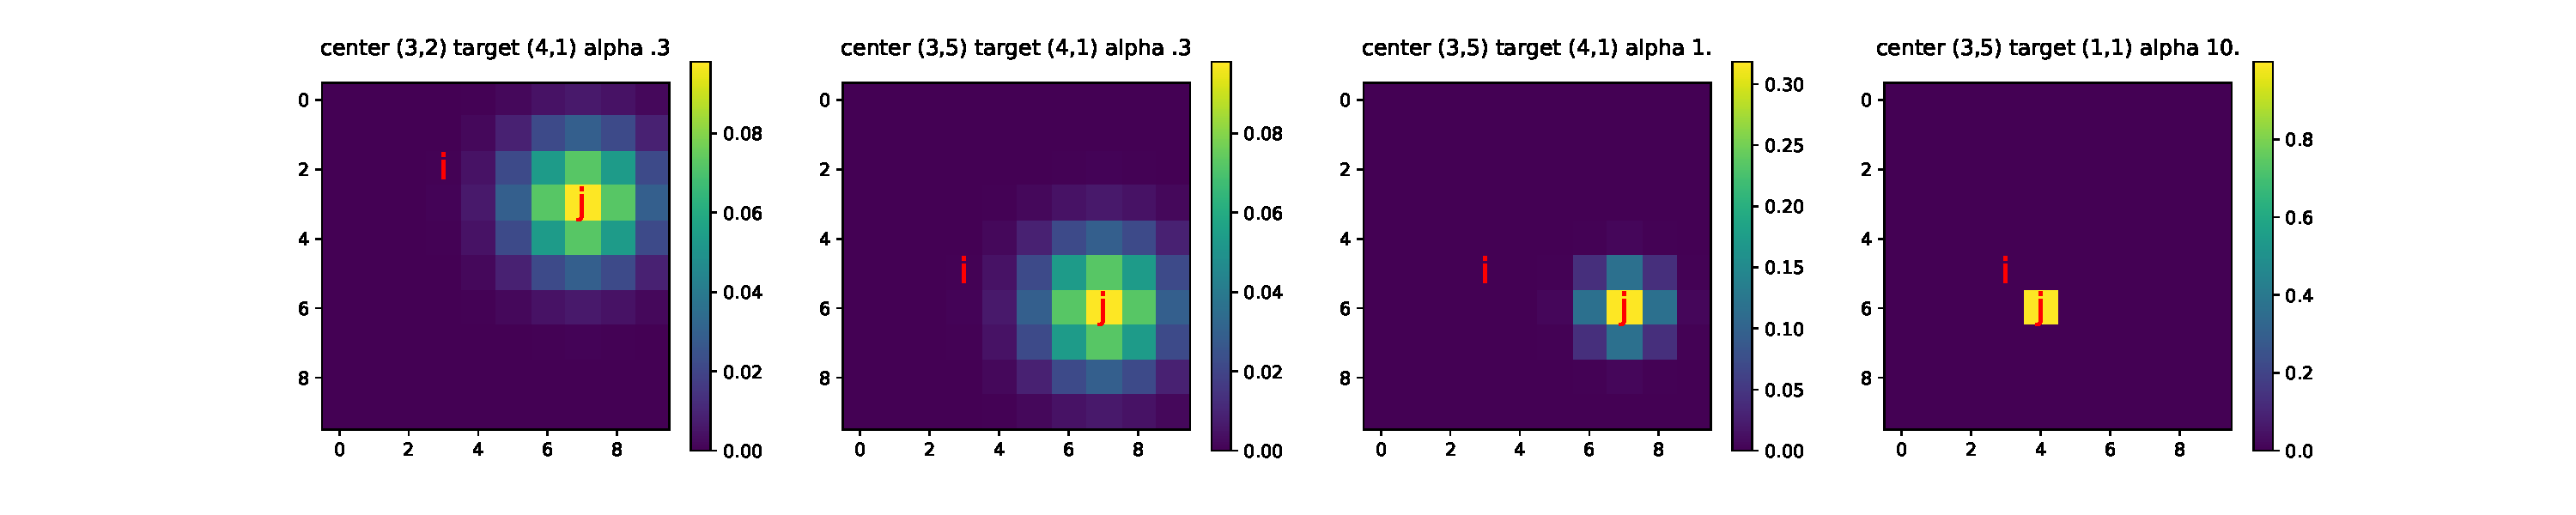
\includegraphics[width=1\linewidth]{plots/conv_attention.pdf}
  \caption{Attention coefficient for different center $i$ and target $j$ with varying $\alpha$ parameters. Target designate the relative position that the head attends to.}
  \label{fig:attention_cnn}
\end{figure}

\paragraph{Discussion.} Some relations can be drawn to RBF kernels centered at the target pixels.
We are expressing a more general form of convolutions where
\emph{(i)} the input pixels do not follow a grid shape but has any pattern and 
\emph{(ii)} the inputs are not single pixels but weighted averages of local patches in the image. 

\paragraph{Simplification.} One further simplification is to remove the constant terms of $\mR_{\Delta}$ because the softmax (renormalization) is shift invariant and constant terms for a head are useless. 


\subsection{Non Isotropic Gaussian}

In this section, we present an extension of the relative positional encoding introduced above
to model non-isotropic Gaussians.

\begin{align}
  f_{\vmu, \mSigma}(\vx) = \exp \left(
    - \frac 1 2
    (\vx - \vmu)^\top \mSigma^{-1} (\vx - \vmu)
  \right)
\end{align}
We drop the normalization factor of the Gaussian distribution as it is replaced by the softmax of the attention mechanism.
The matrix $\mSigma^{-1}$ must be positive semi-definite.
We parametrize it as 
\begin{align}
  \mSigma^{-1} = (\mSigma^{-1/2})^\top\mSigma^{-1/2} = \begin{pmatrix}a & b \\ b & c\end{pmatrix}  
\end{align}
Our goal is to write the exponent as a dot product of two vectors:
\begin{itemize}
  \item one vector $R_\vx$ dependent only on $\vx$, the relative positional encoding,
  \item one vector $\mathbf{t}_h$ dependent only on $\vmu$ and $\mSigma$, the attention head.
\end{itemize}
\begin{align}
  R_\vx &= 
  \begin{pmatrix}
    x_1      & x_2       & x_1      & x_2      & x_1^2   & x_2^2 & x_1 x_2 & 1        & 1         & 1
  \end{pmatrix}\\
  \mathbf{t}_h &= -\frac{1}{2}
  \begin{pmatrix}
    -2a\mu_1 & -2c \mu_2 & -2b\mu_2 & -2b\mu_1 & a       & c     & 2b      & a\mu_1^2 & c\mu_2^2 & 2b\mu_1 \mu_2
  \end{pmatrix}\\
  R_\vx^\top \mathbf{t}_h &=
  -\frac{1}{2} 
  \left[
  a(x_1 - \mu_1)^2 + 2b(x_1-\mu_1)(x_2 -\mu_2) + c(x_2-\mu_2)^2 
  \right]
  = - \frac 1 2 (\vx - \vmu)^\top \mSigma^{-1} (\vx - \vmu)
\end{align}
We can check that setting $b = 0$ and $a=c=\alpha$ recovers the expression of the isotropic Gaussian derived above.

\subsection{Implications to Sinusoid and Learned Positional Encoding} 


\subsection{Exploit Attention on Features?} 
\begin{itemize}

  \item Does the terms (a) (b) (c) allow to condition the CNN filters on the input data?
\end{itemize}


\section{Experiments}
\label{sec:experiments}

We want to validate that not only Transformer architecture can express CNN filters
but that it can also learn such filters with SGD from the data.
%
It has already been shown by \citep{belloAttentionAugmentedConvolutional2019} that 
adding attention features to CNNs can improve performence on Cifar-100 and ImageNet.
%
We want to stick to a fully attentional model, and show that it matches its siblings ResNet of equivalent depth.

\subsection{Performance Against ResNet}

We design a smaller ResNet (i.e. ResNet10) which have similar number of layers as our transformer.
The sizes of the models are displayed in Table~\ref{tab:parameter_size}. 

\begin{table}
  \centering
  \begin{tabular}{cc}
    \toprule
    Models & Number of parameters\\
    \midrule
    ResNet10 & 4.9M\\
    BERT 4 layers & 1.85M\\
    BERT 6 layers & 9.56M \\
    \bottomrule
  \end{tabular}
  \caption{Number of parameters per model.}
  \label{tab:parameter_size}
\end{table}

\begin{figure}[h]
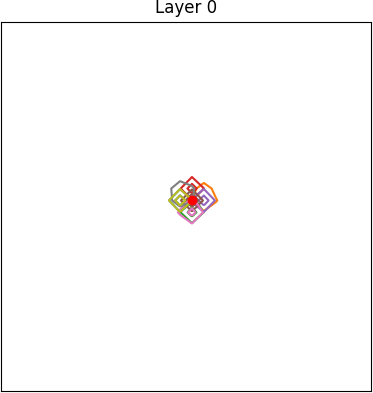
\includegraphics[width=.16\linewidth]{plots/attention/layer_0.png}
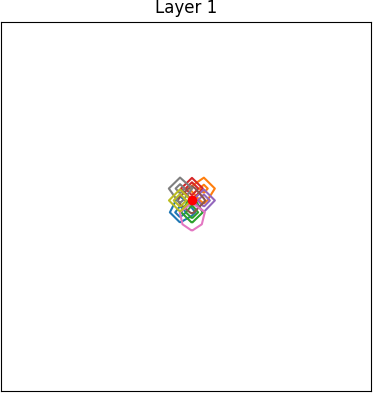
\includegraphics[width=.16\linewidth]{plots/attention/layer_1.png}
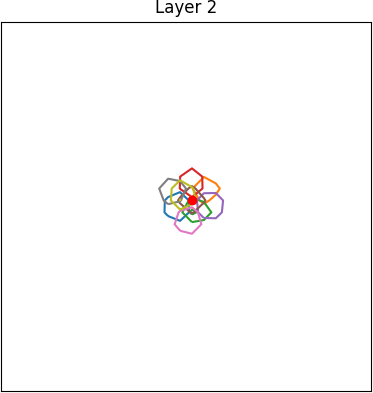
\includegraphics[width=.16\linewidth]{plots/attention/layer_2.png}
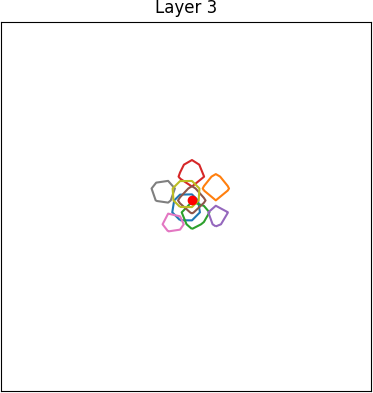
\includegraphics[width=.16\linewidth]{plots/attention/layer_3.png}
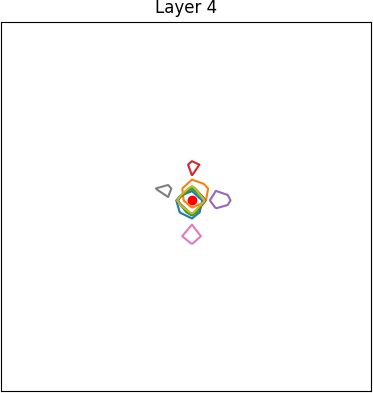
\includegraphics[width=.16\linewidth]{plots/attention/layer_4.png}
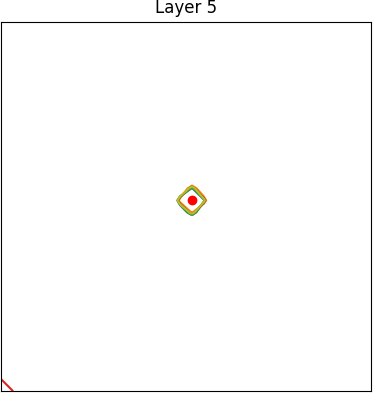
\includegraphics[width=.16\linewidth]{plots/attention/layer_5.png}
\caption{Contours of attention weights per layer for the 6 layers fully attentional model.}
\end{figure}

\begin{figure}[h]
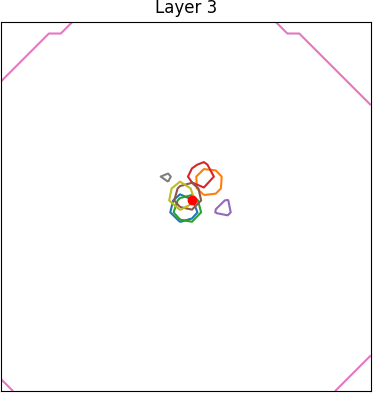
\includegraphics[width=.13\linewidth]{plots/attention_training/layer_3_0.png}
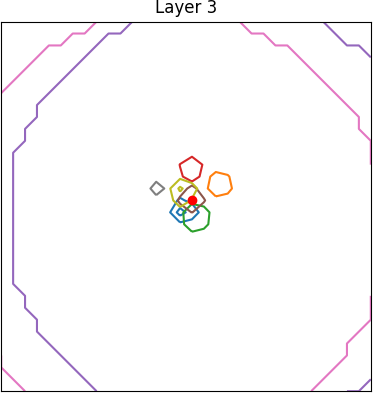
\includegraphics[width=.13\linewidth]{plots/attention_training/layer_3_1.png}
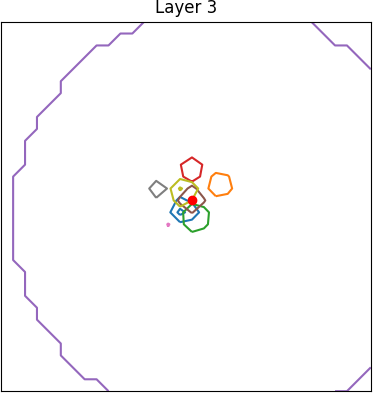
\includegraphics[width=.13\linewidth]{plots/attention_training/layer_3_2.png}
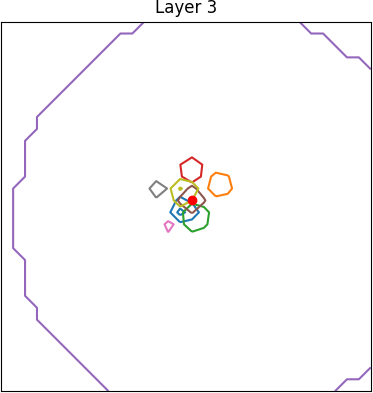
\includegraphics[width=.13\linewidth]{plots/attention_training/layer_3_3.png}
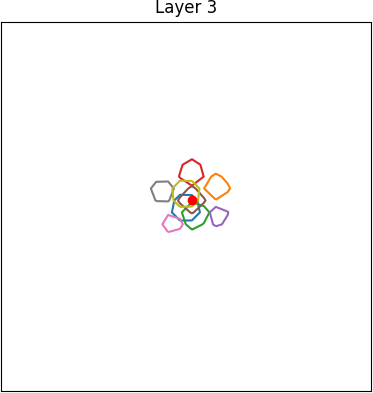
\includegraphics[width=.13\linewidth]{plots/attention_training/layer_3_4.png}
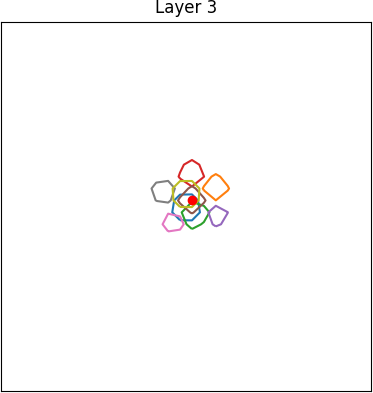
\includegraphics[width=.13\linewidth]{plots/attention_training/layer_3_5.png}
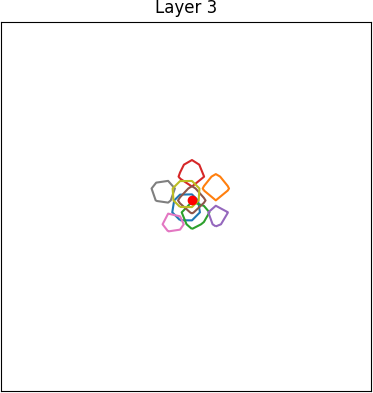
\includegraphics[width=.13\linewidth]{plots/attention_training/layer_3_6.png}
\caption{Contours of attention weights during training (300 epochs) at layer 3.}
\end{figure}

\begin{figure}[h]
  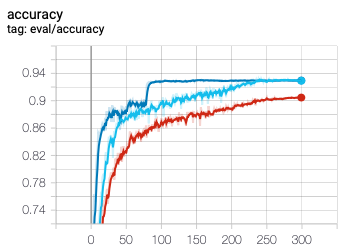
\includegraphics[width=.4\linewidth]{plots/eval_accuracy_plot.png}
  \hfill
  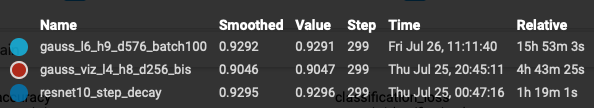
\includegraphics[width=.6\linewidth]{plots/eval_accuracy_legend.png}
  \caption{Evaluation accuracy on CIFAR-10 of a small ResNet and two Gaussian Attention models.}
\end{figure}



\section{Discussion}
\label{sec:discussion}



% \subsubsection*{Author Contributions}
% If you'd like to, you may include  a section for author contributions as is done
% in many journals. This is optional and at the discretion of the authors.

\subsubsection*{Acknowledgments}
Use unnumbered third level headings for the acknowledgments. All
acknowledgments, including those to funding agencies, go at the end of the paper.


\bibliography{bibliography}
\bibliographystyle{iclr2020_conference}

% \appendix
% \section{Appendix}
% You may include other additional sections here. 

\end{document}
